\documentclass[compress]{beamer}
\usepackage{ifthen,verbatim,ulem}

\newcommand{\isnote}{}
\xdefinecolor{lightyellow}{rgb}{1.,1.,0.25}
\xdefinecolor{darkblue}{rgb}{0.1,0.1,0.7}

%% Uncomment this to get annotations
%% \def\notes{\addtocounter{page}{-1}
%%            \renewcommand{\isnote}{*}
%% 	   \beamertemplateshadingbackground{lightyellow}{white}
%%            \begin{frame}
%%            \frametitle{Notes for the previous page (page \insertpagenumber)}
%%            \itemize}
%% \def\endnotes{\enditemize
%% 	      \end{frame}
%%               \beamertemplateshadingbackground{white}{white}
%%               \renewcommand{\isnote}{}}

%% Uncomment this to not get annotations
\def\notes{\comment}
\def\endnotes{\endcomment}

\setbeamertemplate{navigation symbols}{}
\setbeamertemplate{headline}{\mbox{ } \hfill
\begin{minipage}{5.5 cm}
\vspace{-0.75 cm} \small
\end{minipage} \hfill
\begin{minipage}{4.5 cm}
\vspace{-0.75 cm} \small
\begin{flushright}
\ifthenelse{\equal{\insertpagenumber}{1}}{}{Jim Pivarski \hspace{0.2 cm} \insertpagenumber\isnote/\pageref{numpages}}
\end{flushright}
\end{minipage}\mbox{\hspace{0.2 cm}}\includegraphics[height=1 cm]{../cmslogo} \hspace{0.1 cm} \includegraphics[height=1 cm]{../tamulogo} \hspace{0.01 cm} \vspace{-1.05 cm}}

\begin{document}
\begin{frame}
\vfill
\begin{center}
\textcolor{darkblue}{\Large Search for energetic $Z$ bosons from new physics}

\vfill
\begin{columns}
\column{0.3\linewidth}
\begin{center}
\large
\textcolor{darkblue}{Jim Pivarski}
\end{center}
\end{columns}

\begin{columns}
\column{0.3\linewidth}
\begin{center}
\scriptsize
{\it Texas A\&M University}
\end{center}
\end{columns}

\vfill
18 November, 2008

\end{center}
\end{frame}

%% \begin{notes}
%% \item This is the annotated version of my talk.
%% \item If you want the version that I am presenting, download the one
%% labeled ``slides'' on Indico (or just ignore these yellow pages).
%% \item The annotated version is provided for extra detail and a written
%% record of comments that I intend to make orally.
%% \item Yellow notes refer to the content on the {\it previous} page.
%% \item All other slides are identical for the two versions.
%% \end{notes}

\small

\begin{frame}
\frametitle{New Analysis: high $p_T$ $Z$ bosons}
\begin{itemize}\setlength{\itemsep}{0.1 cm}
\item Object-based search for $Z\to\mu\mu$ with unusually high $p_T$
\item \mbox{ }

\vspace{-0.8 cm}
\begin{columns}
\column{0.04\linewidth}

\column{0.46\linewidth}
New particles that are ``heavy versions'' of SM particles can spectroscopically decay to their SM variants by radiating a $Z$

\vspace{0.2 cm}
Example: $q^* \to q \, Z$

\mbox{ }

\column{0.5\linewidth}
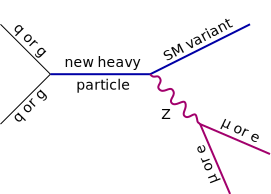
\includegraphics[width=\linewidth]{diagram.png}
\end{columns}

\vspace{-0.8 cm}
\mbox{ }

\item First Stage: only reconstruct the $Z\to\mu\mu$ (later, $ee$)

\item If there's an excess, look at the rest of the event to try to identify the ``SM variant''

\begin{itemize}
\item an energetic jet?
\item a massive jet? (may be $Z\to j j$ or $W\to j j$ if $M_{\mbox{\scriptsize jet}} > 50$~GeV)
\item a lepton?  multiple leptons?
\item missing energy?
\item multiple jets? (David Stuart's analysis)
\end{itemize}

\item Second Stage: if no excess in $Z$-only channel, explicitly
  reconstruct ``SM variants'' in broad categories

\end{itemize}
%% \hspace{-0.83 cm} \textcolor{darkblue}{\Large Outline2}
\end{frame}

\begin{frame}
\frametitle{First Stage: just $Z\to\mu\mu$}
\begin{itemize}\setlength{\itemsep}{0.2 cm}
\item \textcolor{darkblue}{Signal:} two muons with invariant mass near $Z$, no other restrictions
\begin{itemize}
\item Need to be careful about defining isolation around the muons, to
  allow the muons to be arbitrarily close to one another
\end{itemize}

\item \textcolor{darkblue}{Reducible backgrounds:}
\begin{itemize}\setlength{\itemsep}{0.1 cm}
\item muons from jets: no charge correlation, look at \mbox{same-sign sample\hspace{-1 cm}}
\item $Z\to\tau\tau$, $t\bar{t}$, $W^+W^-$: control with dimuon mass sideband
\item cosmic rays: out-of-time and offset vertex control regions
\end{itemize}

\item \textcolor{darkblue}{Irreducible backgrounds:} Standard Model $Z$, $WZ$, and $ZZ$
\begin{itemize}
\item Standard Model $Z$ is likely the most significant background
\end{itemize}

\item Energetic muons have the same efficiency and
  resolution issues as they do in TeV dimuon analysis
\begin{itemize}
\item SM $Z$ distribution not expected to smear much \mbox{due to resolution\hspace{-1 cm}}
\item muon $\vec{p}$ resolution is additionally important for narrowing $Z$ mass peak
  and cutting reducible backgrounds
\end{itemize}
\end{itemize}
\end{frame}

\begin{frame}
\frametitle{Simulation of SM $Z$}
\begin{itemize}
\item Alpgen MC simulation of all \mbox{$pp \to N j \, Z$ and $pp \to q\bar{q} \, N j \, Z$ diagrams\hspace{-1 cm}}
\begin{itemize}
\item where ``$j$'' is a parton ($q$ or $g$)
\item for all $N$ from 0 to 6 (inclusive sum of channels)
\item ignore jets and jet-merging, $Z \to \mu\mu$ \mbox{is good at generator-level\hspace{-1 cm}}
\end{itemize}

\item Also study realistic distribution by smearing the generator-level muons with resolution($p_T$, $\eta$) distributions from \mbox{CMSSW (``Fast{\it \underline{er}}Sim'')\hspace{-1 cm}}
\end{itemize}

Effective cross-section of $pp \to X \, Z \to X \, \mu\mu$ per 20~GeV bin versus $Z$ $p_T$

\vspace{0.15 cm}
\mbox{ } \hfill \includegraphics[height=0.9\linewidth, angle=90]{insensitivity_to_misalignment.pdf} \hfill \mbox{ }
\end{frame}

\begin{frame}
\frametitle{Benchmark model: $q^* \to q \, Z$}
\begin{itemize}
\item Excitation of quarks due to substructure on a scale $\Lambda \approx M_{q^*}$
\item Clearly visible above SM $Z$ distribution
\item $\Lambda$ = 1~TeV should be visible in 100~pb$^{-1}$ \mbox{(these are 10~TeV collisions)\hspace{-1 cm}}
\item Misalignment doesn't broaden peaks much ($p_T$ distributions are already rather broad)
\end{itemize}

\only<1>{\includegraphics[height=\linewidth, angle=90]{excited_quarks_ideal.pdf}}
\only<2>{\includegraphics[height=\linewidth, angle=90]{excited_quarks_misaligned.pdf}}
\end{frame}

\begin{frame}
\frametitle{Would this find a graviton?}
\begin{itemize}
\item ${\mathcal B}(G^* \to ZZ)$ = $2 \times {\mathcal B}(G^* \to \mu\mu)$, but ${\mathcal B}(Z \to \mu\mu)$ = 3.4\%
\item Nevertheless, $ZZ$ mode remains a good way to distinguish \mbox{$G^*$ from $Z'$\hspace{-1 cm}}
\item Would a search for only one of the two $Z$ bosons \mbox{be significant? ($c=0.1$)\hspace{-1 cm}}
\end{itemize}

\includegraphics[height=\linewidth, angle=90]{gravitons_ideal.pdf}

\begin{itemize}
\item An explicit $G^* \to ZZ \to \mu\mu jj$ search (where $jj$ can be a fat jet) would be more sensitive
\end{itemize}
\end{frame}

\begin{frame}
\frametitle{Overlapping muons?}
\small

\begin{columns}
\column{0.7\linewidth}
\begin{itemize}
\item If the $Z$ is very boosted, would its daughter muons overlap?
\begin{itemize}
\item TeV muons shower in the muon system: delta rays could in principle overlap
\end{itemize}
\item But they don't: 1--2~TeV $Z$ bosons have clearly-separated muons (angle $>$ 5$^\circ$), and lower momentum muons are cleaner than this
\end{itemize}
\column{0.3\linewidth}
\includegraphics[width=\linewidth]{opening_angle_1500.pdf}
\end{columns}

\begin{columns}
\column{0.2\linewidth}
\mbox{Hit distribution\hspace{-0.5 cm}} around the two muons

\vspace{0.2 cm}
normalized to \mbox{muon separation\hspace{-0.5 cm}}

\vspace{0.2 cm}
including hits not associated with tracks
\column{0.8\linewidth}
\includegraphics[height=\linewidth, angle=90]{hit_distribution_from_muons.pdf}
\end{columns}
\end{frame}

%% \section*{First section}
%% \begin{frame}
%% \begin{center}
%% \Huge \textcolor{blue}{First section}
%% \end{center}
%% \end{frame}

\begin{frame}
\frametitle{Steps in First Stage analysis}
\begin{enumerate}

\item Feasibility studies $\surd$
\begin{itemize}
\item \mbox{\sout{Inclusive SM $Z$ background distribution from Alpgen for high $p_T$}\hspace{-1 cm}}
\item \sout{Quantify discovery potential with a benchmark model}
\item \sout{Check for overlapping muon showers in full CMSSW}
\end{itemize}

\item Study reducible backgrounds in large MC productions
\begin{itemize}
\item Determine optimal muon isolation and $Z$ mass cuts
\item Practice same-sign and sideband background estimations
\end{itemize}

\item Alpgen in full CMSSW?  At least validate Pythia \mbox{inclusive $p_T$ spectrum\hspace{-1 cm}}
\begin{itemize}
\item $Z$ efficiency and muon charge misassignment versus $p_T$
\item Sensitivity to misalignment
\end{itemize}

\item Refinements
\begin{itemize}
\item Define analysis in PAT, make sure PAT objects are sufficient
\item Quantify theoretical uncertainties in SM $Z$ distribution (PDFs)
\item Calculate $Z$ efficiency from data-driven muon efficiencies
\item Split search into $\eta$ regions?
\item Define blinding procedure?  ($p_T > 250$-$300$~GeV is new)
\item Limit calculations for signature and benchmark models
\end{itemize}

\end{enumerate}
\end{frame}

\begin{frame}
\frametitle{Conclusions}
\begin{itemize}\setlength{\itemsep}{0.25 cm}
\item Heavy versions of SM particles would radiate energetic $Z$
  bosons instead of photons to decay neutrally to their SM versions
\begin{itemize}
\item Excited quark model is a good benchmark \mbox{(excited leptons, too)\hspace{-1 cm}}
\end{itemize}
\item Simplest search, asking only for the $Z\to\mu\mu$, is feasible
  and would find the benchmark
\item $G^* \to ZZ \to \mu\mu jj$ can't be identified by the $\mu\mu$
  alone: must also reconstruct $jj$ (either in the Second Stage of
  this analysis or an exclusive search)
\item I'm moving on to full-MC studies
\item CDF and D0 $Z$ samples reach up to $p_T \approx 250$-$300$~GeV
  in 1~fb$^{-1}$

  \vspace{0.1 cm}
  We should see about 20$\times$ as many SM $Z$ bosons in
  that energy range in 100~pb$^{-1}$ at 10~TeV
\end{itemize}
\label{numpages}
\end{frame}

\end{document}
